%\documentclass[letterpaper, 10 pt, conference]{ieeeconf}  % Comment this line out
                                                          % if you need a4paper
\documentclass[a4paper, 10pt, conference]{ieeeconf}      % Use this line for a4
                                                          % paper

\IEEEoverridecommandlockouts                              % This command is only
                                                          % needed if you want to
                                                          % use the \thanks command
\overrideIEEEmargins
% See the \addtolength command later in the file to balance the column lengths
% on the last page of the document



% The following packages can be found on http:\\www.ctan.org
\usepackage{graphicx}
\usepackage{listings}
\usepackage{xcolor}

\definecolor{mGreen}{rgb}{0,0.6,0}
\definecolor{mGray}{rgb}{0.5,0.5,0.5}
\definecolor{mPurple}{rgb}{0.58,0,0.82}

\lstdefinestyle{CStyle}{  
    commentstyle=\color{mGreen},
    keywordstyle=\color{magenta},
    numberstyle=\tiny\color{mGray},
    stringstyle=\color{mPurple},
    basicstyle=\footnotesize,
    breakatwhitespace=false,         
    breaklines=true,                 
    captionpos=b,                    
    keepspaces=true,                 
    numbers=left,                    
    numbersep=5pt,                  
    showspaces=false,                
    showstringspaces=false,
    showtabs=false,                  
    tabsize=2,
    language=C
}


\title{\LARGE \bf
Feasability of a Benchmarking Framework for Context-Switching in RTOS
}

\author{Julien Gomez -- julien.gomez@student.uclouvain.be
\\ Trong-Vu Tran -- trong-vu.tran@student.uclouvain.be}


\begin{document}

\maketitle
\thispagestyle{empty}
\pagestyle{empty}


%%%%%%%%%%%%%%%%%%%%%%%%%%%%%%%%%%%%%%%%%%%%%%%%%%%%%%%%%%%%%%%%%%%%%%%%%%%%%%%%
%\begin{abstract}
%\end{abstract}


%%%%%%%%%%%%%%%%%%%%%%%%%%%%%%%%%%%%%%%%%%%%%%%%%%%%%%%%%%%%%%%%%%%%%%%%%%%%%%%%
\section{INTRODUCTION}
% Explain the motivation
One of the goal of our thesis is to write a framework able to compute the context switching time between different tasks of an application.
Commonly, the context switching is measured using an oscilloscope.
However, that kind of hardware is costly and not everyone can have access to such device.
In order to compute the context switching time without an oscilloscope, we developped a framework.
Its implementation and its usage are discussed in this paper.

The first section describes the framework we built on different OS's.
The second section talks about reference measurements we performed to assess our framework performances.
Section 3 shows the impact of the framework on the application performances.


\section{\label{sec:bench}BENCHMARKING FRAMEWORK}

Every time a task runs, it calls the \texttt{bench\_ping} function providing its process ID.
The framework then checks if a context switch happened by comparing the active process ID with the previous one.
If the IDs do not match, it means that the active task has changed and the framework will compute the elapsed time and print it.

The source code of the benchmarking framework implemented in Contiki can be found in listing \ref{lst:code}.

\begin{lstlisting}[style=CStyle, label={lst:code}, caption={Source code of the benchmarking framework implemented in Contiki}]
/**
 * Struct that stores benchmarking information.
 * 
 * previous_id: The id of the previous thread that performs a ping;
 * new_id: The id of the current thread that has performed a ping;
 * current_time: the timer
 */
struct BContext {
  uint32_t previous_id;
  uint32_t new_id;
  clock_time_t current_time;
} bench_context;


void bench_ping(uint32_t id) {
  // Save the new id
  bench_context.new_id = id;
  // Save the current time
  // Check for switching context
  if (!check_change()) {
    bench_context.current_time = RTIMER_NOW(); // Ticks
  }
}

int check_change(void) {
  if(bench_context.new_id != bench_context.previous_id) {
    // Compute the difference
    clock_time_t previous = bench_context.current_time;
    clock_time_t current = RTIMER_NOW();
    clock_time_t result = current - previous;

    // Keep the previous id for log
    uint32_t previous_id = bench_context.previous_id;
    // Change previous_id to new_id
    bench_context.previous_id = bench_context.new_id;

    bench_context.current_time = RTIMER_NOW(); // Ticks

    printf("[BENCH_CONTEXT_SWITCHING] %lu %lu %lu\n", previous_id, bench_context.new_id, result);
    
    return 1; // Change occurs
  }
  return 0; // No change
}
\end{lstlisting}

\section{\label{sec:ref}REFERENCE MEASUREMENT}
The first step is to perform a measurement that will be used as a reference point.
This reference point will be used to assess if our benchmarking framework compute the correct context switching values and if it adds any overhead during the process.

In order to perform this measurement, we used the Pocket Science Lab device from PSLab.io.

\begin{figure}[!h]
    \centering
    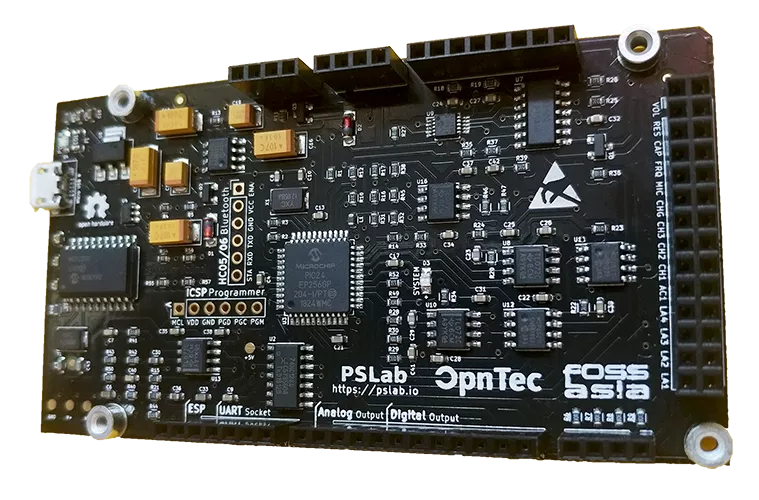
\includegraphics[scale=0.2]{pslab.png}
    \caption{Pocket Science Lab device}
    \label{fig:pslab}
\end{figure}

This board comes with a built-in oscilloscope that we used to perform our measurements.
A real oscilloscope could have been used but, in the context of this work, no such hardware was available.

Our experience was made on a simple application.
The application consists of two tasks.
The first task sets a GPIO up, waits for 1ms then sets the same GPIO down.
The other task does the same but with an other GPIO.
Using the collaborative scheduling, each task runs after the other.

In order to have a collaborative scheduling, we used Contiki to run the application.

Using the Pocket Science Lab device, we were able to measure the voltage of the two GPIO's used by the application.
In the Fig.\ref{fig:ref}, we can see each GPIO being up and down for 1ms.
We can also see during a small amount of time that none of the GPIO's are up.
The context switch happens during this period.
No task is in the foreground during this time.


\begin{figure}[!h]
    \centering
    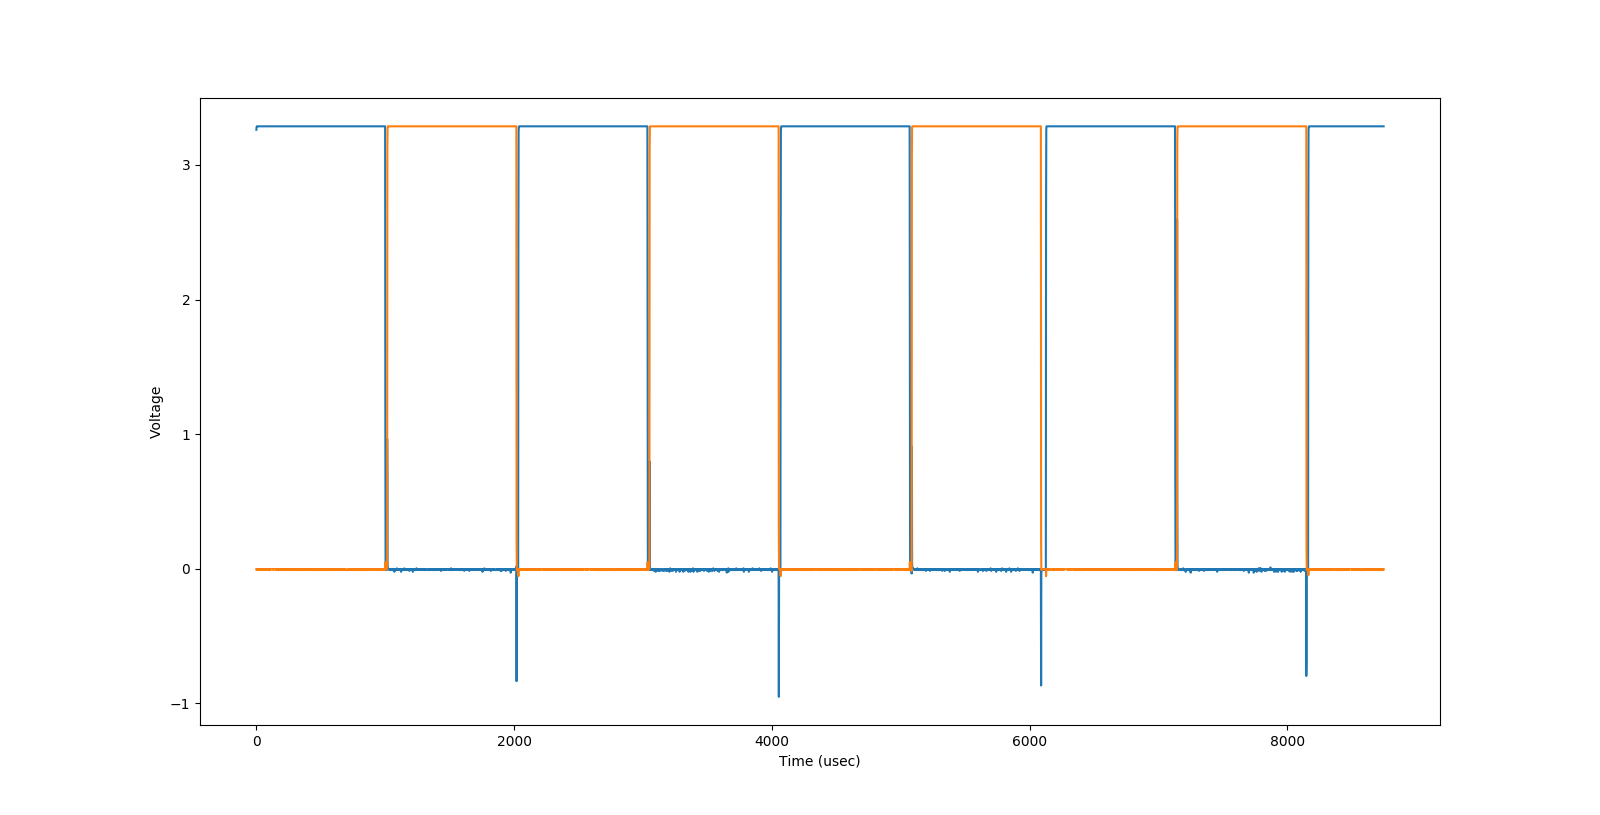
\includegraphics[scale=0.2]{ref.png}
    \caption{Reference measurement made with PSLab}
    \label{fig:ref}
\end{figure}



Using this reference, we can see how our framework change the performances of the application.
Ideally, the time between two tasks should not change with our framework.

\section{EMBEDDED FRAMEWORK OVERHEAD}

Using the Pocket Science Lab device, we did the same experience described in section \ref{sec:ref}.
Fig.\ref{fig:framework_overhead} shows the results of the experiment.

\begin{figure}[!h]
    \centering
    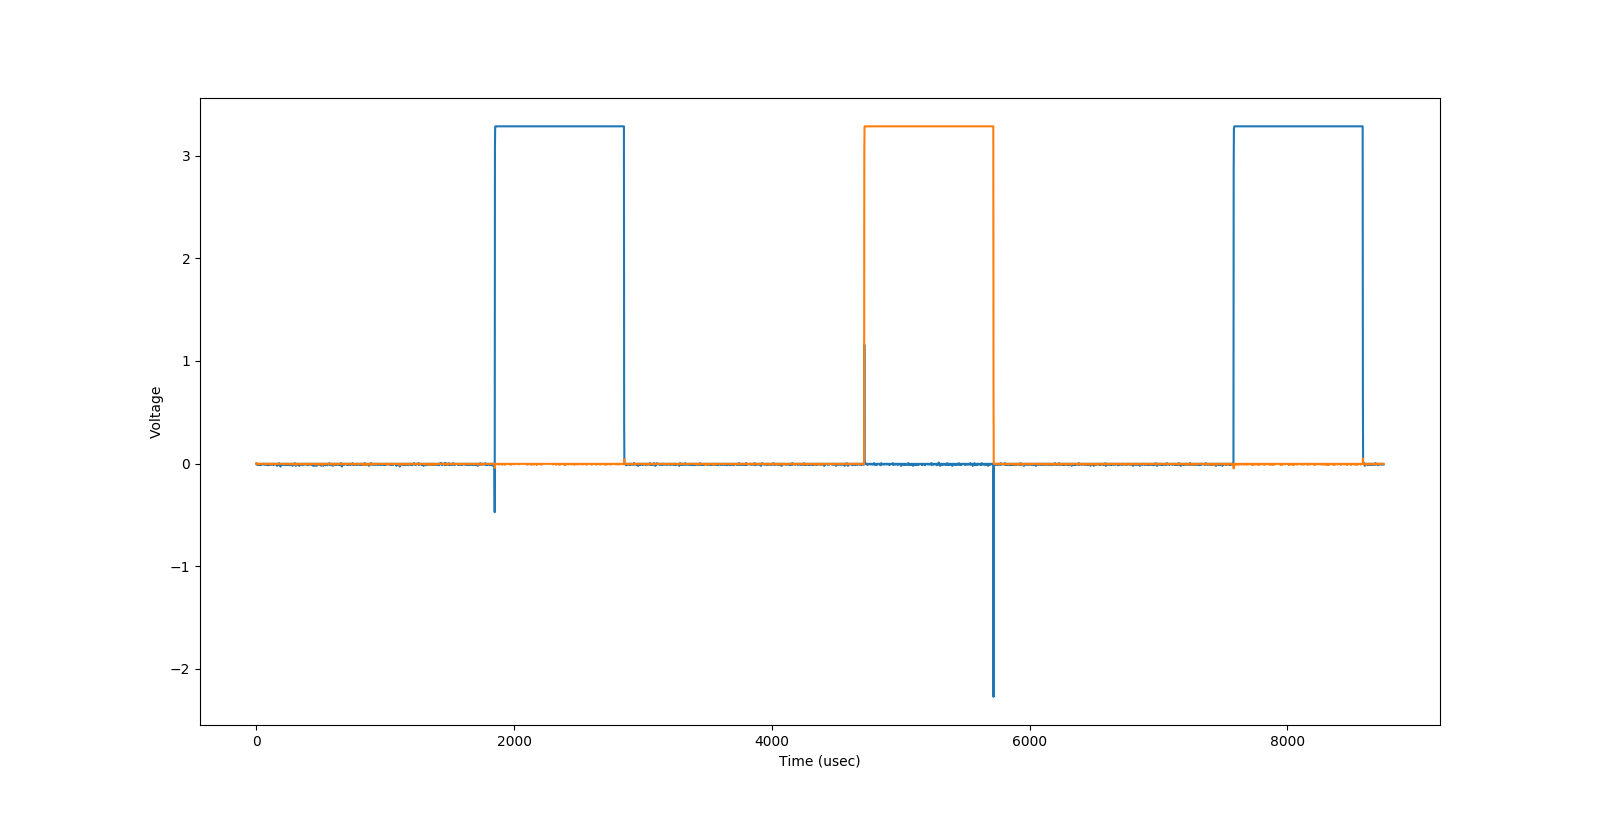
\includegraphics[scale=0.2]{framework_overhead.png}
    \caption{Embedded Framework Overhead measured with PSLab}
    \label{fig:framework_overhead}
\end{figure}

Table \ref{table:context_switching_times} compares the context switching time with and without our benchmarking framework.
We can see that the framework adds a huge overhead.


\begin{table}[!h]
    \centering
    \caption{Context switching times measured with the Pocket Science Lab device with and without the framework}
    \begin{tabular}{llll}
        \cline{2-4}
        & Mean ($\mu s$) & Median ($\mu s$) & Mode ($\mu s$) \\ \cline{2-4}
        Without the framework & 18.47 & 15.75 & 15.75 \\
        With the framework & 1864.33 & 1863.75 & 1863.75
    \end{tabular}
    \label{table:context_switching_times}
\end{table}

\section{PYTHON ALTERNATIVE}
Considering that our benchmarking framework adds a large overhead, we tried a new alternative.

The idea is to perform every computational task on a computer instead of the board.
Using the UART protocol over USB, the board sends a single byte containing the process ID that is read by a Python script on the computer.
In the same way described in section \ref{sec:bench} with the framework, the Python script computes the context switching.

The motivations for using this alternative are:
\begin{itemize}
    \item Sending one byte of data over USB with UART have a smaller impact than computing the context switching time locally on the board;
    \item Heavy computational tasks of the framework are done on the computer and not on the board;
    \item Using Python3.7, we can achieve a time precision at the nanosecond.
\end{itemize}

A first drawback of this method is that the communication between the board and the computer using UART over USB adds a large amount of milliseconds that is counted in the context switching time by the Python script.
A solution would be to compute this overhead added by the UART protocol and remove it from the computed values.

\section{CONCLUSION}
We have tried to create a benchmarking framework to compute the context switching time of a RTOS using different methodologies.
We have started by implementing the framework inside the RTOS.
We predicted that an overhead due to the serial output and the computational tasks made in the board would be present.
However, the overhead was bigger than expected.

Moreover, the capabilities of the board are not big enough to reach high timing precision.
The next step of this work is to externalize the computation using Python and UART over USB.

\addtolength{\textheight}{-12cm}   % This command serves to balance the column lengths
                                  % on the last page of the document manually. It shortens
                                  % the textheight of the last page by a suitable amount.
                                  % This command does not take effect until the next page
                                  % so it should come on the page before the last. Make
                                  % sure that you do not shorten the textheight too much.

%%%%%%%%%%%%%%%%%%%%%%%%%%%%%%%%%%%%%%%%%%%%%%%%%%%%%%%%%%%%%%%%%%%%%%%%%%%%%%%%



%%%%%%%%%%%%%%%%%%%%%%%%%%%%%%%%%%%%%%%%%%%%%%%%%%%%%%%%%%%%%%%%%%%%%%%%%%%%%%%%



%%%%%%%%%%%%%%%%%%%%%%%%%%%%%%%%%%%%%%%%%%%%%%%%%%%%%%%%%%%%%%%%%%%%%%%%%%%%%%%%


%%%%%%%%%%%%%%%%%%%%%%%%%%%%%%%%%%%%%%%%%%%%%%%%%%%%%%%%%%%%%%%%%%%%%%%%%%%%%%%%

\end{document}
